\section{Results}

When discussing the results, I refer to the algorithm-interface pairs with acronyms for brevity:
NM (Nelder-Mead),
BO (Bayesian Optimization).

\begin{figure}
  \centering
  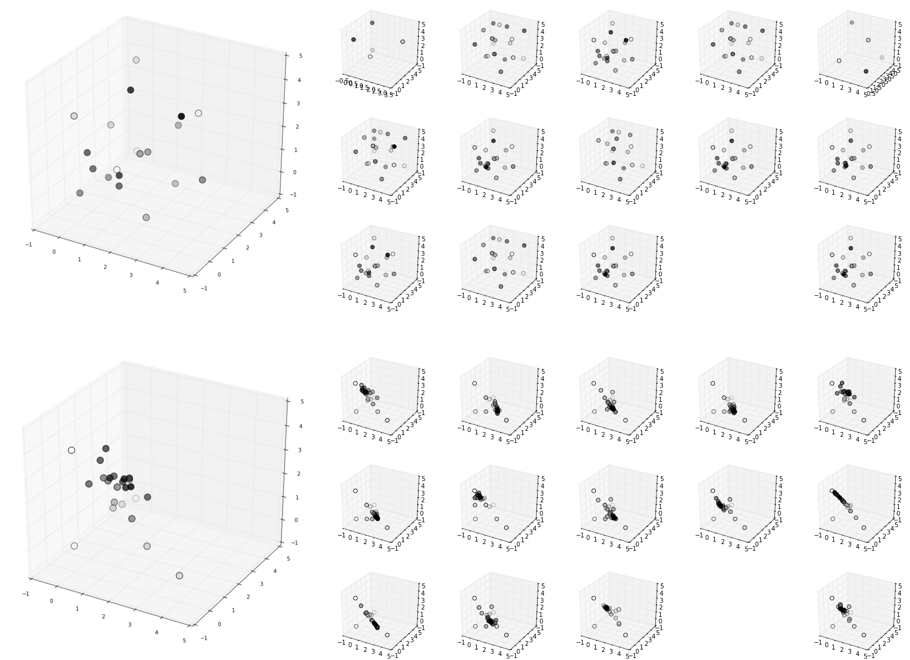
\includegraphics[width=0.45\textwidth]{figures/scatters}
  \caption{%
    Coverage of the parameter space by each method.  
    An exemplar of each group is shown on the left. 
    The top row is Bayesian Optimization, and the bottom row is Nelder-Mead.
    Small multiples of the points for all participants are shown to the right of the enlarged images.
    To show the procession of points, the first point a user proposes is white, and the last one black.
    Each new point proposed by the algorithm fades gradually through grey to black.
    The Nelder-Mead method appears to pull in its vertices linearly.
    Bayesian Optimization, however, appears to randomly jump over the larger space.
    \andrew{Probably break up this image into two columns, across the top of the page.}
  }\label{fig:coverage}
\end{figure}

\begin{figure}
  \centering
  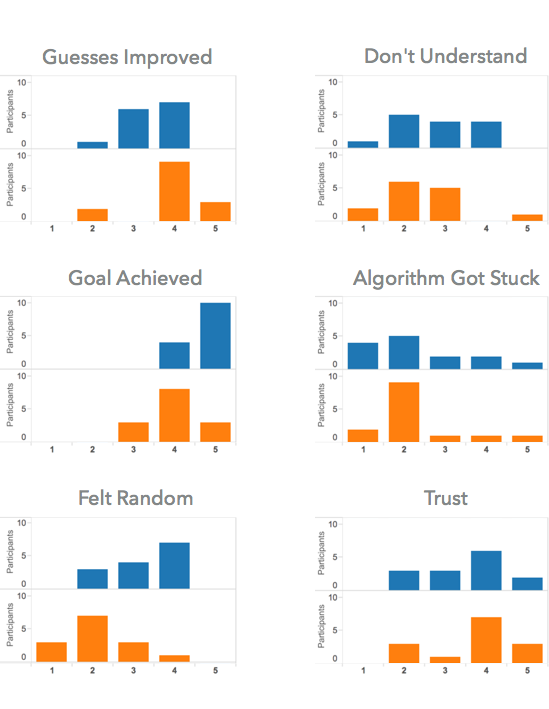
\includegraphics[width=0.4\textwidth]{figures/feedback}
  \caption{%
    Qualitative feedback
  }\label{fig:feedback}
\end{figure}

Let's talk about parameter space coverage.
The first points sampled are white, and they fade to black as you get more samples.
On the left is a typical participant's exploration of the space with BO---it's all over the place, but looks like it heads towards the left side.
\andrew{Look up how to assess and compare Likert scale data.
The current analysis just isn't comprehensive enough.}
\andrew{The values of parameter space coverage are\ldots{}}

Each line represents the new points that were proposed to each participant, and its height is the distance of that point from the goal.
If we're just looking at the new points that each one proposes, BO is all over the map.
But for NM, these distances started high, and usually ended up getting closer and closer to the goal.
But these are just new points.
Which one got the participant's favorite point closer to the goal, faster?
\andrew{The average distances over time for each algorithm are\ldots{}}

\begin{figure}
  \centering
  \begin{subfigure}[b]{0.23\textwidth}
    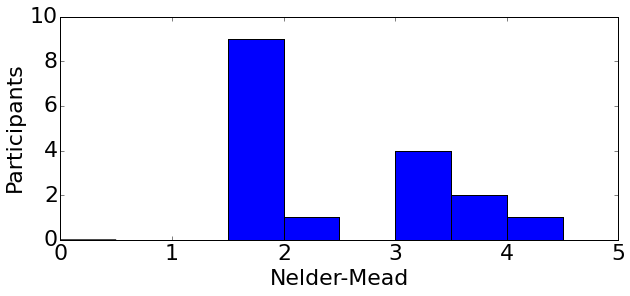
\includegraphics[width=\textwidth]{figures/bestfits_nm}
  \end{subfigure}
  \begin{subfigure}[b]{0.23\textwidth}
    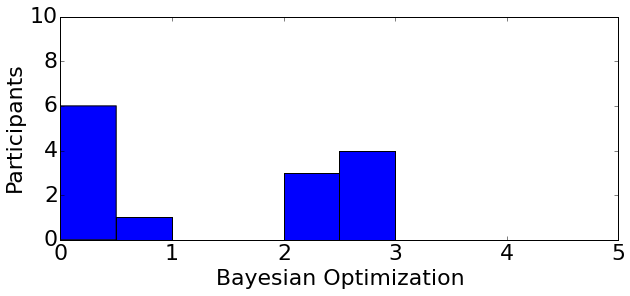
\includegraphics[width=\textwidth]{figures/bestfits_bo}
  \end{subfigure}
  \caption{Best fits for Nelder-Mead~\andrew{Increase the text size.}}\label{fig:bestfits}
\end{figure}

If we just look at the end points (Figure~\ref{fig:bestfits}).
BO got users closer to their intended goal more frequently than the NM method.
Part of this may have been due to the sample points chosen.
And at the same time, some configurations that look very similar are actually very far apart in the parameter space.
This is all something I'll have to sort out in a follow-up study.

Participants were more likely to say that the Bayesian Optimization felt random, but also more adamant that they one they marked as best was very close to the goal.
While the simplex seemed more likely to improve, it was also more likely to get stuck.
